

\chapter{Introducción específica} % Main chapter title

\label{Chapter2}

%----------------------------------------------------------------------------------------
%	SECTION 1
%----------------------------------------------------------------------------------------
Todos los capítulos deben comenzar con un breve párrafo introductorio que indique cuál es el contenido que se encontrará al leerlo.  La redacción sobre el contenido de la memoria debe hacerse en presente y todo lo referido al proyecto en pasado, siempre de modo impersonal.

\section{Requerimientos}
...

\section{Tecnologias de hardware utilizadas}

\subsection{ESP32}

ESP32 es una serie de microcontroladores de bajo costo y bajo consumo creado y desarrollado por Espressif Systems embebido en un chip con Wi-Fi integrado (2.4 GHz band) y Bluetooth de modo dual. Emplea dos cores Xtensa® 32-bit LX6 CPU. Incluye interruptores de antena integrados, balun de RF, amplificador de potencia, amplificador de recepción de bajo ruido, filtros, un co-procesador ULP (Ultra Low Power),  módulos de administración de energía y varios periféricos.
La placa utilizada para el desarrollo del presente trabajo es ESP32-WROOM-32D.

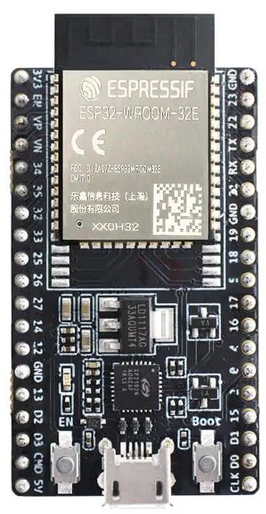
\includegraphics[scale=0.25]{esp32}


\subsection{DHT11}

El DHT11 es un sensor digital de temperatura y humedad relativa de bajo costo y fácil uso. Integra un sensor capacitivo de humedad y un termistor para medir el aire circundante, y muestra los datos mediante una señal digital en el pin de datos (no posee salida analógica). Utilizado en aplicaciones académicas relacionadas al control automático de temperatura, aire acondicionado, monitoreo ambiental en agricultura y más.

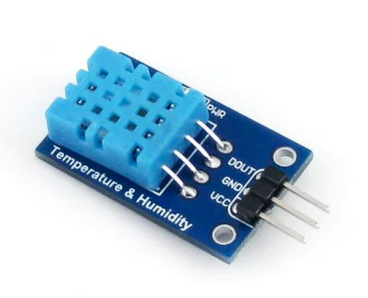
\includegraphics[scale=0.25]{dht11}


\subsection{BMP280}

El BMP280 es un sensor de presión barométrica absoluta, especialmente factible para aplicaciones móviles. Sus reducidas dimensiones y su bajo consumo permiten su implementación en dispositivos alimentados por batería como teléfonos móviles, módulos GPS o relojes. Se basa en la tecnología comprobada de sensor de presión piezorresistivo de Bosch que ofrece alta precisión y linealidad, así como estabilidad a largo plazo y alta robustez de EMC. El dispositivo está optimizado en términos de consumo de energía, puede ser utilizado con I2C o SPI, y ofrece una precisión absoluta de ±1 hPa en lectura de presión y ±1,0 °C para temperatura. Además, dada la precisión del dispositivo y al hecho de que la presión cambia con la altitud, también puede usarse como un altímetro con una precisión de ± 1 metro.


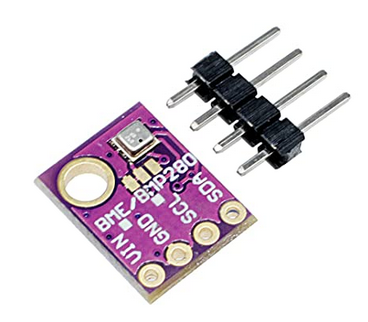
\includegraphics[scale=0.25]{bmp280}

\subsection{Fotoresistor}



El fotoresistor es una resistencia eléctrica que varía su valor en función de la cantidad de luz que incide sobre su superficie. Cuanto mayor sea la intensidad de luz que incide en la superficie del LDR o fotoresistor menor será su resistencia y en cuanto menor sea la luz que incida sobre éste mayor será su resistencia. 
Cuando el fotoresistor no está expuesto a radiaciones luminosas, los electrones están firmemente unidos en los átomos que lo conforman, pero cuando sobre él inciden radiaciones luminosas, esta energía libera electrones con lo cual el material se hace más conductor, y de esta manera disminuye su resistencia. Las resistencias LDR solamente reducen su resistencia con una radiación luminosa situada dentro de una determinada banda de longitudes de onda. El fotoresistor construido con sulfuro de cadmio son sensibles a todas las radiaciones luminosas visibles y las construidas con sulfuro de plomo solamente son sensibles a las radiaciones infrarrojas.


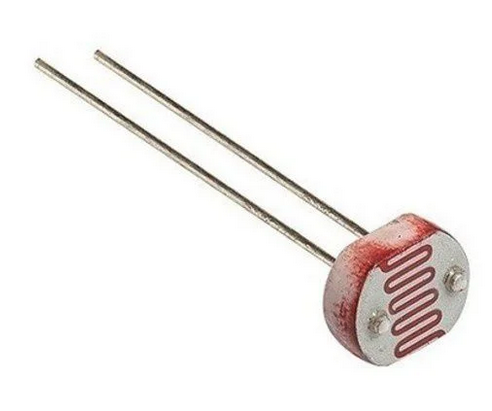
\includegraphics[scale=0.25]{fotoresistor}


\subsection{Joystick analógico}

El módulo de joystick analógico está construido sobre el montaje de dos potenciómetros en un ángulo de 90 grados. Los potenciómetros están conectados a una palanca corta centrada por resortes. Este módulo produce una salida de alrededor de 2,5 V cuando inicialmente se encuentra en posición de reposo (en el centro), mientras que en el trayecto del desplazamiento de la palanca hará que la salida varíe de 0V a 5V
dependiendo de su dirección X e Y. Al conectar este módulo a un microcontrolador se puede leer un valor de alrededor de 512 en su posición de reposo mientras que al moverlo cambia entre 0 y 1023 dependiendo de su posición.


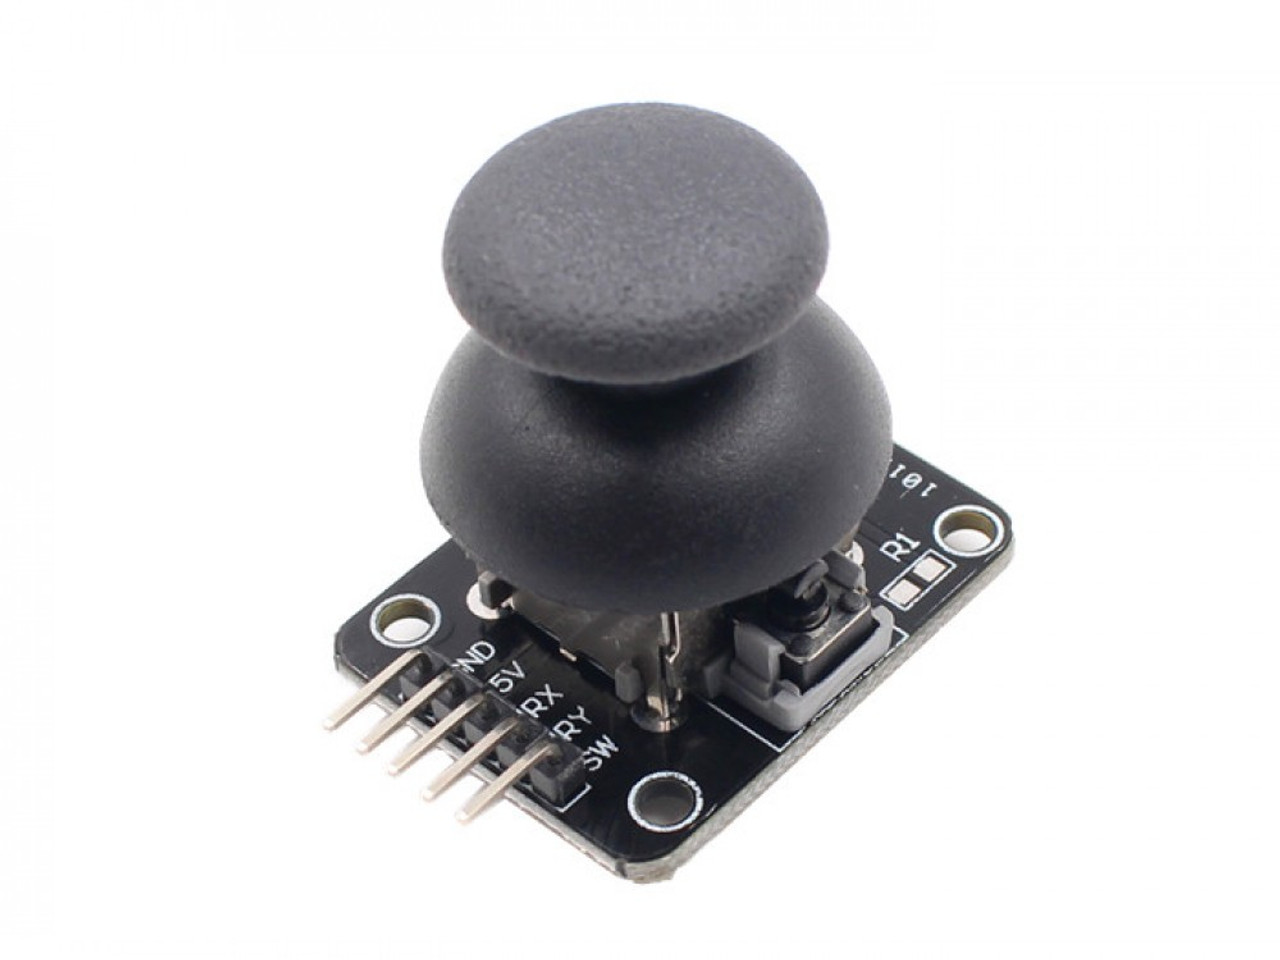
\includegraphics[scale=0.15]{joystick}

\subsection{Display}
...pendiente...

\subsection{Motores}
...pendiente...

\subsection{Integrados y otras utilidades}
...pendiente...


\section{Tecnologias de software utilizadas} 

\subsection{ESP-IDF}

Espressif proporciona recursos básicos de hardware y software para ayudar a los desarrolladores de aplicaciones a realizar sus ideas utilizando el hardware de la serie ESP32. El framework de software de Espressif está destinado al desarrollo de aplicaciones de Internet de las cosas (IoT) con Wi-Fi, Bluetooth, administración de energía y varias otras características del sistema.
Sus componentes son:
\begin{enumerate}
	\item Toolchain para compilar el codigo para ESP32
	\item Build tools - con utilidades como CMake y Ninja para construir la aplicación completa para ESP32
	\item ESP-IDF que esencialmente contiene la API de desarrollo (software base y librerias complementarias) para ESP32 y scripts para ejecutar Toolchain



\includegraphics[scale=0.25]{espressif}

\end{enumerate}

\subsection{Docker}

Docker es un proyecto de código abierto que automatiza el despliegue de aplicaciones dentro de contenedores de software, proporcionando una capa adicional de abstracción y automatización de virtualización de aplicaciones en múltiples sistemas operativos.​ Docker utiliza características de aislamiento de recursos del kernel Linux, tales como cgroups y espacios de nombres (namespaces) para permitir que "contenedores" livianos independientes se ejecuten en paralelo de manera aislada evitando la sobrecarga de iniciar y mantener máquinas virtuales.


\includegraphics[scale=0.15]{docker}

\subsection{Visual Studio Code}

Visual Studio Code es un editor de código fuente desarrollado por Microsoft para Windows, Linux, macOS y Web. Incluye soporte para la depuración, control integrado de Git, resaltado de sintaxis, finalización inteligente de código, fragmentos y refactorización de código. 


\includegraphics[scale=0.15]{vscode}

\subsection{Ubuntu}
Ubuntu es una distribución Linux basada en Debian GNU/Linux y patrocinado por Canonical, que incluye principalmente software libre y de código abierto. Puede utilizarse en ordenadores y servidores, está orientado al usuario promedio, con un fuerte enfoque en la facilidad de uso y en mejorar la experiencia del usuario. 


\includegraphics[scale=0.25]{ubuntu}

...